
\begin{figure}
    \centering
    \begin{subfigure}[b]{0.48\textwidth}
        \centering
        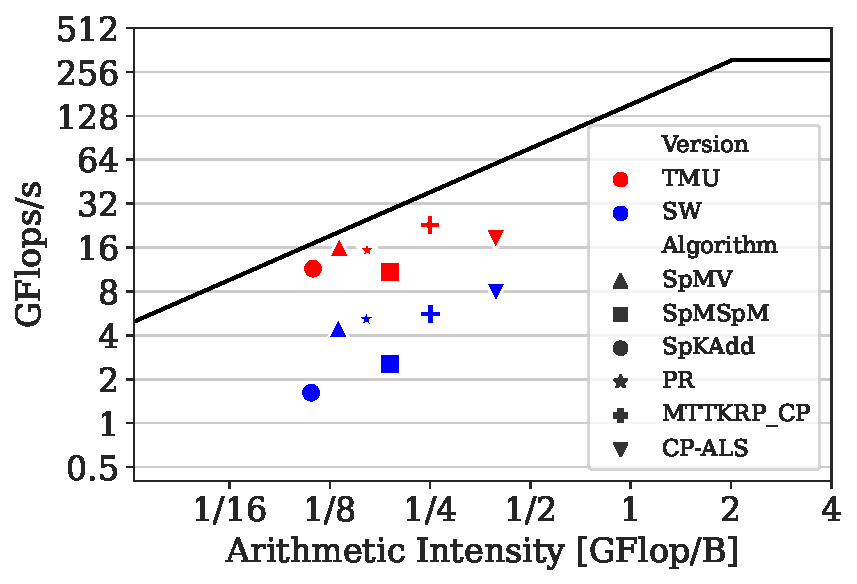
\includegraphics[width=\textwidth]{img_roofline_all.pdf}
        \vspace{-0.5cm}
        \caption{Geomean}
        \label{fig:tmu-scientific-roofline-geomean}
    \end{subfigure}
    \centering
    \begin{subfigure}[b]{0.48\textwidth}
        \centering
        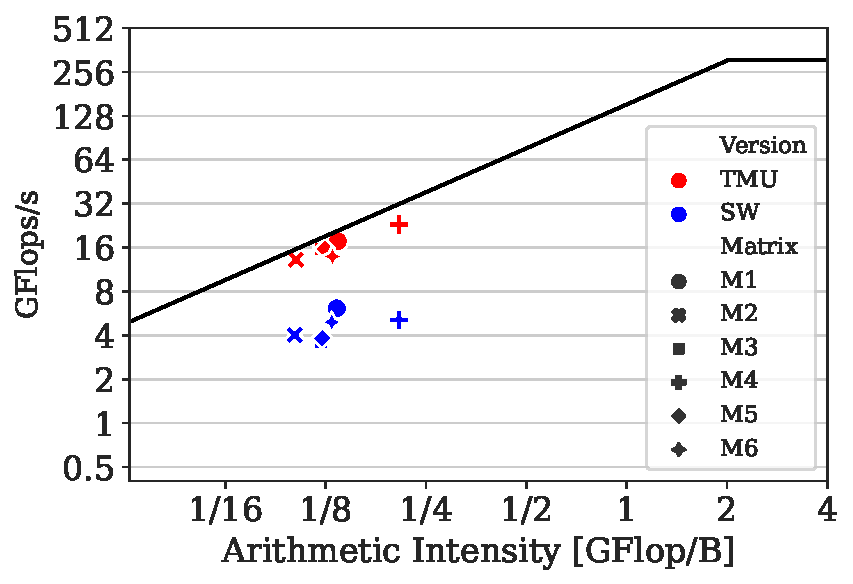
\includegraphics[width=\textwidth]{img_roofline_spmv.pdf}
        \vspace{-0.5cm}
        \caption{SpMV}
        \label{fig:tmu-scientific-roofline-spmv}
    \end{subfigure}
    \centering
    \begin{subfigure}[b]{0.48\textwidth}
        \centering
        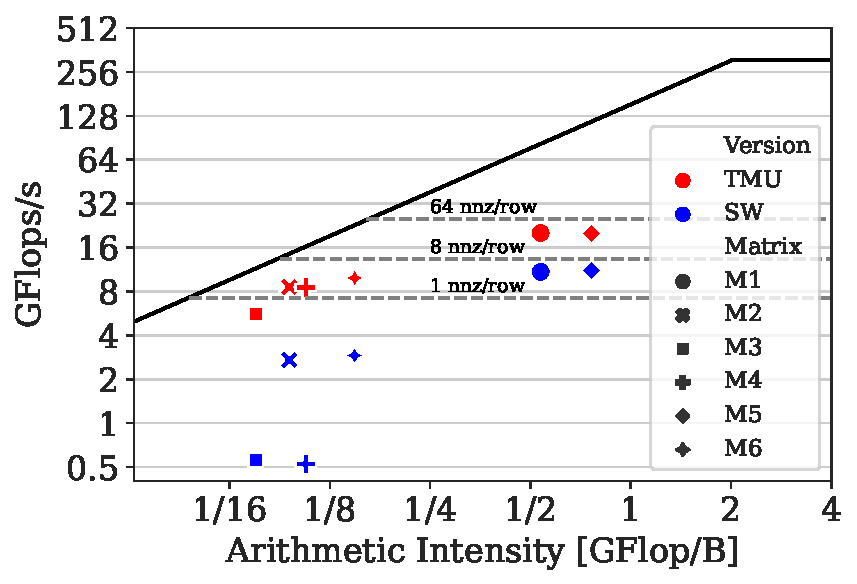
\includegraphics[width=\textwidth]{img_roofline_spgemm.pdf}
        \vspace{-0.5cm}
        \caption{SpMSpM}
        \label{fig:tmu-scientific-roofline-spmspm}
    \end{subfigure}
    \centering
    \begin{subfigure}[b]{0.48\textwidth}
        \centering
        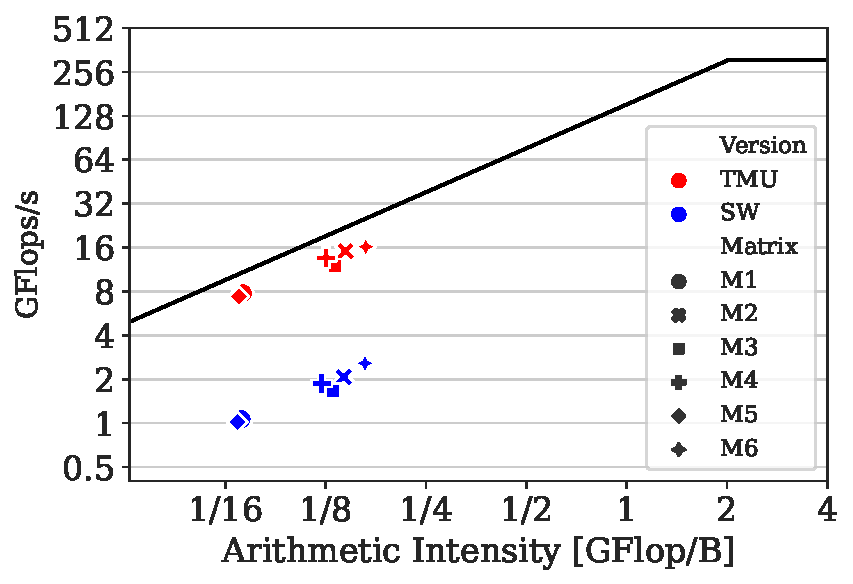
\includegraphics[width=\textwidth]{img_roofline_spkadd.pdf}
        \vspace{-0.5cm}
        \caption{SpKAdd}
        \label{fig:tmu-scientific-roofline-spkadd}
    \end{subfigure}
    \caption[Roofline models of a CPU and DAE processor on scientific kernels.]{Roofline analysis of the traditional CPU baseline and the proposed DAE processor on scientific sparse kernels. Both systems use the simulated multicore configuration in \Cref{tab:tmu-dae-system-specs}; the DAE processor augments each core with a TMU, while the baseline executes the optimized software implementations described in \Cref{sec:tmu-scientific-methodology}. Each point reports one execution, with operational intensity on the x-axis and achieved floating-point throughput on the y-axis; diagonal and horizontal roofs denote the memory-bandwidth and peak-compute limits, respectively. \Cref{fig:tmu-scientific-roofline-geomean} reports geomeans across inputs for each workload, while \Cref{fig:tmu-scientific-roofline-spmv,fig:tmu-scientific-roofline-spmspm,fig:tmu-scientific-roofline-spkadd} report all inputs for SpMV, SpMSpM, and SpKAdd; the dashed ceilings in \Cref{fig:tmu-scientific-roofline-spmspm} show idealized SpMSpM limits for fixed nonzeros per row. Overall, the TMU does not change operational intensity, but it moves executions closer to the relevant bandwidth or compute roof by improving memory-level parallelism and reducing traversal and merging overheads.}
    \label{fig:tmu-scientific-rooflines}
\end{figure}
